\documentclass[11pt,a4paper]{article}

% Packages
\usepackage[utf8]{inputenc}
\usepackage[margin=0.8in]{geometry}
\usepackage{graphicx}
\usepackage{amsmath}
\usepackage{booktabs}
\usepackage[hyphens]{url}
\usepackage[breaklinks=true]{hyperref}
\usepackage{enumitem}
\usepackage{caption}
\usepackage{subcaption}
\usepackage{float}
\usepackage{tikz}
\usetikzlibrary{positioning}

% Title information
\title{\textbf{Advanced Natural Language Processing} \\
       \large Assignment 4: Transformer Architecture}
\author{Lucia Welther, Matrikelnummer: 835106}
\date{\today}

\begin{document}

\maketitle

% ============================================================
\section{Architecture}
% ============================================================
\begin{figure}[H]
\centering
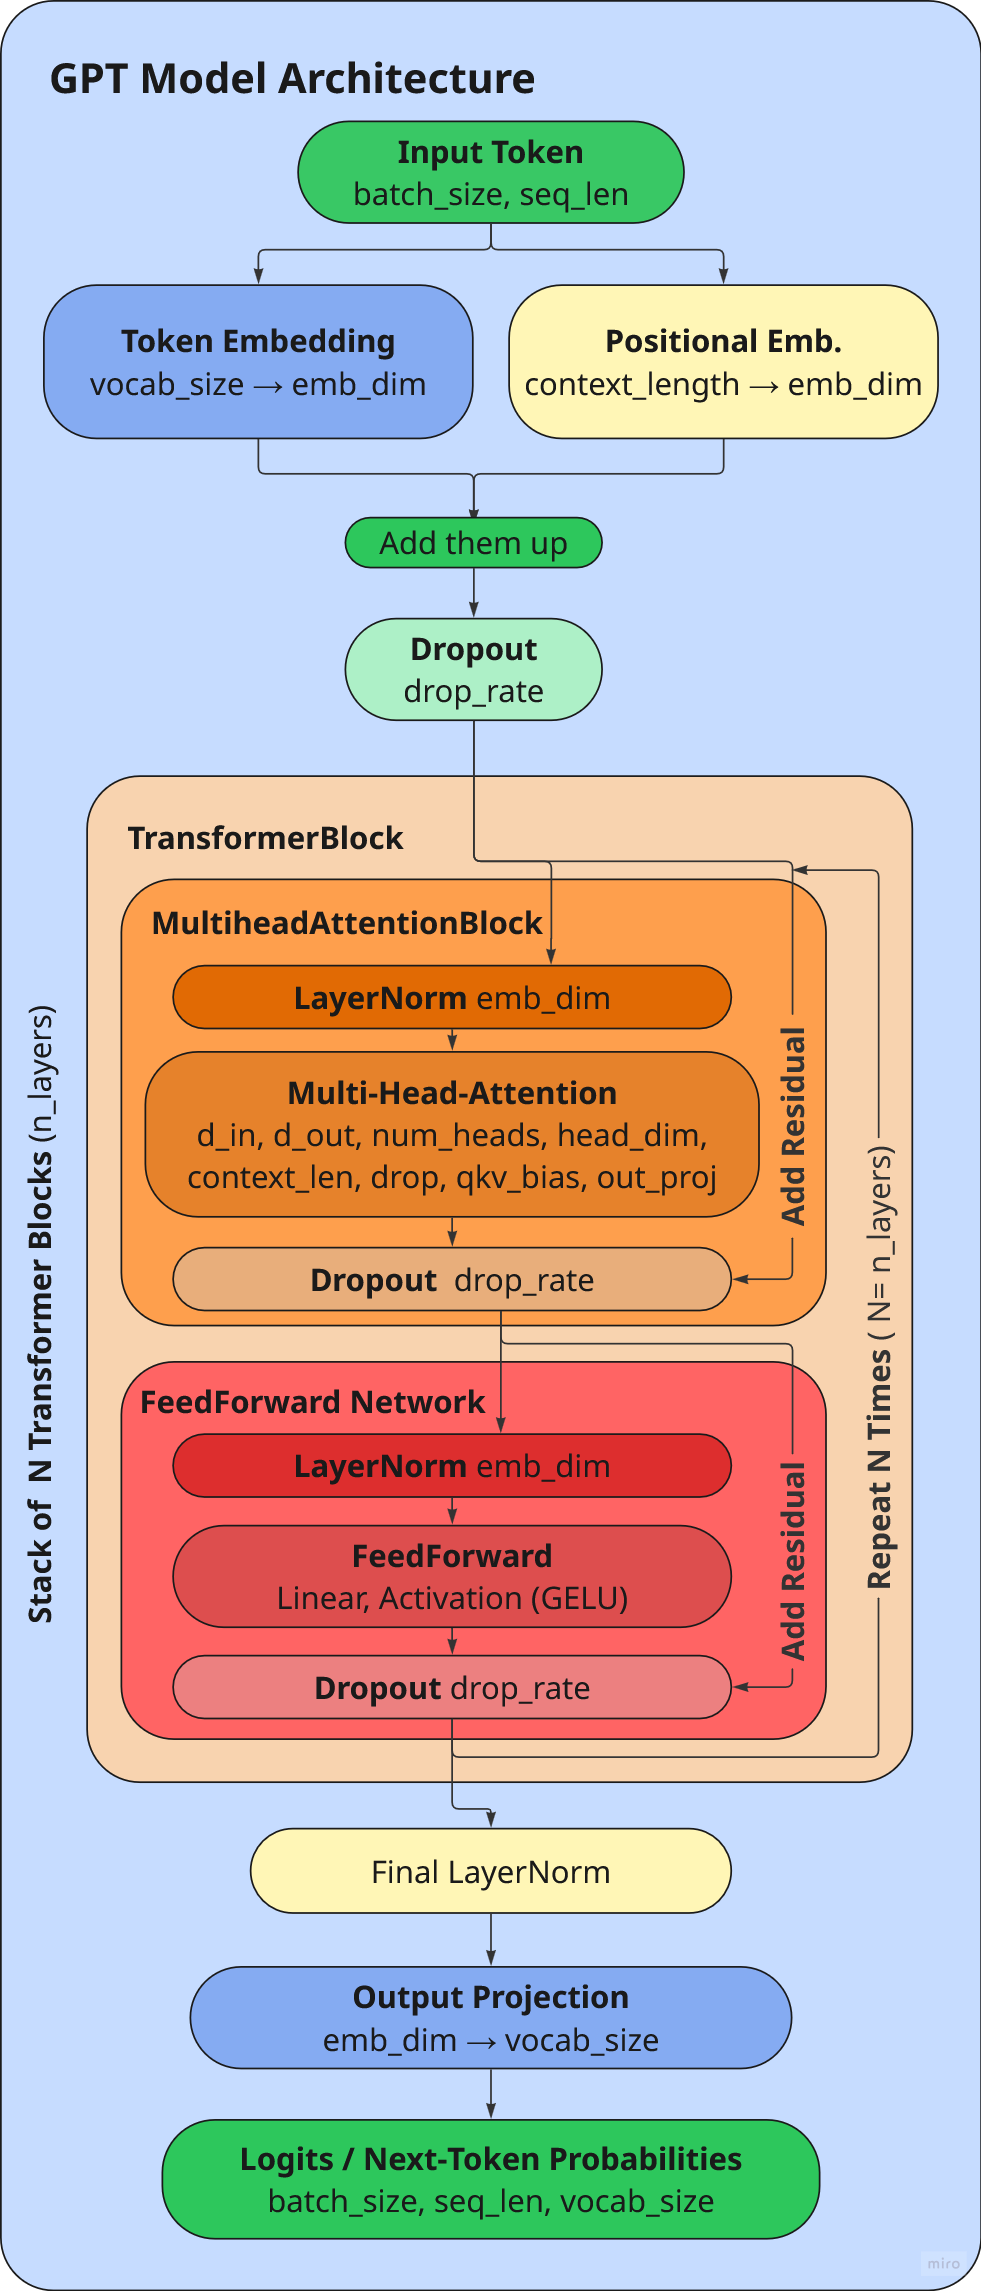
\includegraphics[width=0.45\textwidth]{image.png}
\caption{GPT Model Architecture}
\label{fig:gpt_architecture}
\end{figure}

\subsection{Description of Architecture}
In Figure~\ref{fig:gpt_architecture} the GPT model is shown. A sequence of token IDs is mapped to dense vectors by a 
token embedding (\texttt{vocab\_size} $\rightarrow$ \texttt{emb\_dim}) and a positional embedding (\texttt{context\_length} 
$\rightarrow$ \texttt{emb\_dim}); the two embeddings are summed and regularized with dropout. The resulting tensor of shape 
(batch, seq\_len, \texttt{emb\_dim}) is processed by a stack of $N$ identical TransformerBlocks.

Each TransformerBlock performs:
\begin{enumerate}
  \item Pre‑LayerNorm on the input.
  \item Multi‑head causal self‑attention with $n\_heads$ (head dimension $=$ \texttt{emb\_dim} / $n\_heads$). The attention output is 
  projected, dropped out, and added to the residual connection.
  \item Pre‑LayerNorm on th eoutput from Mulit-headattention Block
  \item Feed‑forward network with GELU activation: \texttt{emb\_dim} $\rightarrow$ $4\cdot$\texttt{emb\_dim} $\rightarrow$ 
  GELU $\rightarrow$ \texttt{emb\_dim}, then dropout and a residual add.
\end{enumerate}

After all layers have been passed through, a final LayerNorm and a linear projection cretae logits/ probabilities over the vocabulary for next‑token prediction. 

\section{Evaluate the Model}

\begin{figure}[H]
\centering
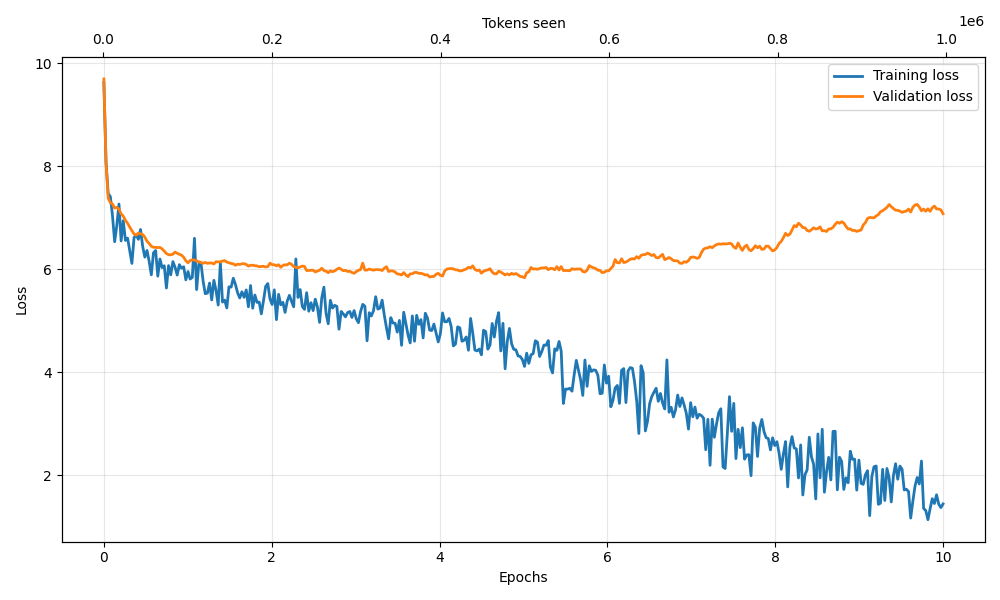
\includegraphics[width=0.8\textwidth]{LossBaseline.png}
\caption{GPT Model Loss Plot}
\label{fig:Loss_Plot}
\end{figure}


In the Figure~\ref{fig:Loss_Plot} you can see how the training loss in contantly dropping over the 10 epochs, while the validation loss is first dropping as fasta s the training loss
, then in a slowr pace until epoch 4, until the loss increases again after. This shows that the model is overfitting to the trainig data, performing well and and always improving on the training data 
but it does not improve in generalizing on the unseen validation data.

During training the output created changed during the epochs. In the first 4 epochs the model generated only one or two new words: ``My beloved Sister, and the''.
Only after longer sequenes are generated. In Epoch 5, 6 and 7 the model got stuck in repeating word sequences and repeating white spaces: ``... the most  the most beautiful and  the most the most the most  the ...'' (Epoch 5).
With each epoch the repeating word sequences got longer. In Epoch 8 the model stopped repeating the same sequences. Thes generated sequence of words, did not 
sound natural nor was grammatical. For the last episodes the sequences read more naturally but still do not have any sentimantic value.

\subsection{Perplexity}


Table~\ref{tab:perplexity} presents the perplexity results for the two test corpora (Frankenstein, Automata). 
The model has a perplexity of 207.8 on Frankenstein, which can be translated into high uncertainty. 
The die\_automata corpus rached even worse results. The perplexity is extremely high (883,024.9), 
meaning that the model assigns probabilities close to zero to most tokens. 
This extreme difference is probalby due to the mismatch in langaue (German vs. English). With the model being trained on english text, 
it generelized very badly on german text (Die Automate).
Training the model on German Text would improve the perplexity on german test corpora.

\begin{table}[H]
\centering
\caption{Perplexity evaluation on test corpora}
\label{tab:perplexity}
\begin{tabular}{lrrr}
\toprule
\textbf{Test Corpus} & \textbf{Tokens Evaluated} & \textbf{Avg. NLL} & \textbf{Perplexity} \\
\midrule
frankenstein\_short.txt & 599 & 5.34 & 207.80 \\
die\_automata.txt & 12,470 & 13.69 & 883,024.94 \\
\bottomrule
\end{tabular}
\end{table}


\section{Decoding}
\subsection{Implementation}

\textbf{Greedy Decoding (already implemented Baseline)}:
The baseline \texttt{generate\_text\_simple()} always selects the token with maximum probability at each step.
\textbf{Top-k Sampling}:
Implementation inspired by: Ansil, M. B. (2025, January 5).
The decode\_1 function keeps only the $k$ most probable tokens, renormalizes, and samples: Sort logits descending, keep top $k$, 
Mask remaining logits to $-\infty$ and Apply softmax and sample from distribution.
$k=50$ and temperature $T=1.0$ were used as default.

\textbf{Nucleus (Top-p) Sampling}:
Implementation inspired by: Ansil, M. B. (2025, January 5).
The decode\_2 function samples from the smallest set of tokens whose cumulative probability exceeds threshold $p$: Sort logits descending, 
Compute cumulative probabilities, Keep tokens while $\sum p_i \leq p$, Mask rest to $-\infty$ and sample.
$p=0.9$ was used as default.

\subsection{Comparison}

\textbf{Greedy decoding output:}
\begin{quote}
\textit{My beloved Sister, and "You will doubtless?"  "If you, dear Margaret, that I am not, that you have been so much: you are not, that the monster?" "Devratitude. If you have been, that you,} \\
(Gets stuck in repetition loop)
\end{quote}

\textbf{Top-k sampling output ($k=50$):}
\begin{quote}
\textit{My beloved Sister, but not a inspired me.  "If you," said he hasably from thank you, what these friends with a pretty not be:."   "Dear, that the stranger was so many years, and the very unlike of}
\end{quote}

\textbf{Nucleus sampling output ($p=0.9$):}
\begin{quote}
\textit{My beloved Sister, I gazed and impassle with you, and said, hated on you; you alone my heart."    "This is you how more "EL--"Dev need you in my; you will befitting kindness;}
\end{quote}

\begin{itemize}
    \item \textbf{Greedy}: Deterministic but prone to repetition loops
    \item \textbf{Top-$k$}: Introduces diversity; fixed $k$ may include unlikely tokens or exclude likely ones
    \item \textbf{Top-$p$}: Dynamically adjusts candidate pool based on probability mass, often producing more natural variation
\end{itemize}

% ============================================================
\section{Hyperparameter Experiments}
% ============================================================
\textbf{GPT-2 Small (124M)}\\
With parameters: ``emb\_dim'': 768, ``n\_layers'': 12, ``n\_heads'': 12, ``epochs'': 10

\begin{quote}
\textit{
My beloved Sister, and "You will doubtless?"  "If you, dear Margaret, that I am not, that you have been so much: you are not, that the monster?" "Devratitude. If you have been, that you,
} \\
\end{quote}

\textbf{GPT-2 Medium (355M)}\\
With parameters: ``emb\_dim'': 1024, ``n\_layers'': 24, ``n\_heads'': 16, ``epochs'': 8
\begin{quote}
\textit{
My beloved Sister, and   "I have not to the s of the s of the s of the s of the s of the the monster and s of the s of the  s of the s of
} \\
\end{quote}

\begin{figure}[H]
\centering
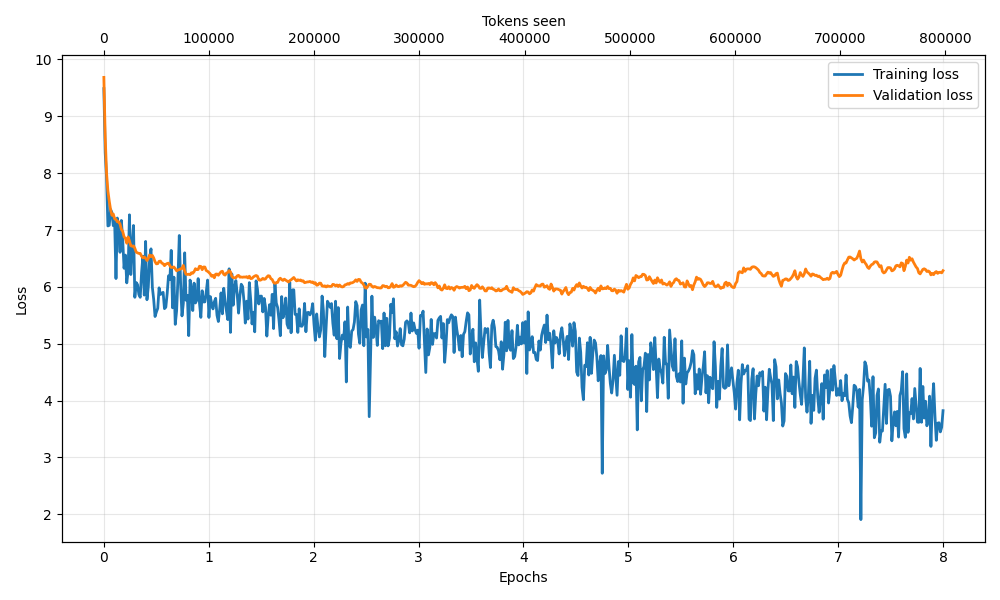
\includegraphics[width=0.8\textwidth]{LossMedium.png}
\caption{GPT Model Loss Plot: gpt2 medium (355M)}
\label{fig:Loss_Plot_medium}
\end{figure}

I used fewer epochs for the medium model to save time and reduce complexity. 
The performance of the medium model was comparable to the small model after 4 iterations, 
but both models did not show optimal performance. The medium model also struggled with generating 
coherent sequences and got stuck in a sequence repetition loop (like the small model in earlier epochs). Interestingly, up until the 
last epoch, the medium model frequently produced only one word after the starting context.

The medium model, with its larger number of parameters, requires more training 
data and epochs to fully converge. But time contrainst made it impossible to train.

In the loss plot for the medium model, a similar behavior to the small model can be observed. 
The training loss decreases steadily, while the 
validation loss remains relatively constant and even increases slightly towards the end, indicating overfitting. 

The larger model parameters, did not run on my computers cpu, so I do not have results for this. I would guess that the performance would not improve with too many and big parameters.
To improve the model I would improve the trianing data to be longer and more complex in vocabulary and language for the model to learn more complex laguage patterns.
% ============================================================
\section{Pretrained vs. From-Scratch Comparison}
\begin{quote}
\textit{
My beloved Sister, I am so sorry for your loss. I am so sorry for your loss. I am so sorry for your loss. I am so sorry for your loss. I am so sorry for your loss. I am so sorry for your loss. I am
} \\
\end{quote}

The pretrained GPT-2 model generates grammatically correct sentences that are coherent and fluent but 
the output gets stuck in repeating patterns, as seen in the repeated phrase "I am so sorry for your loss." 
This shows that while the pretrained model has strong language fluency, it may rely too heavily on high-probability tokens, leading to repetitive outputs.

In comparison, the self-trained model produces outputs with less grammatical correctness and fluency but
the choice of words and sentence structure occasionally aligns better with the training data's style. 
Looking at earlier epochs in training of the self-trained model repetition can also be seen.

\section{Submission}


\newpage
\section*{References}

Ansil, M. B. (2025, January 5). \textit{From randomness to precision: How top-k, top-p, temperature, and beam 
search shape text generation}. Medium. Retrieved from 
\url{https://medium.com/@ansilproabl/from-randomness-to-precision-how-top-k-top-p-temperature-and-beam-search-shape-text-generation-d1f50b5220e2}


\end{document}